\setchapterimage{fig_00}
\chapter*{TD \arabic{cptTD} \\ 
Assistance pour le maniement de charges dans l’industrie -- \ifprof Corrigé \else Sujet \fi}

\addcontentsline{toc}{section}{TD \arabic{cptTD} : Assistance pour le maniement de charges dans l’industrie -- \ifprof Corrigé \else Sujet \fi}

\iflivret \stepcounter{cptTD} \else
\ifprof  \stepcounter{cptTD} \else \fi
\fi
\setcounter{question}{0}

\marginnote{Concours Centrale Supelec TSI 2017.}
%\marginnote{\UPSTIcompetence[2]{B2-07}\UPSTIcompetence[2]{C2-03}}
\begin{marginfigure}
\centering
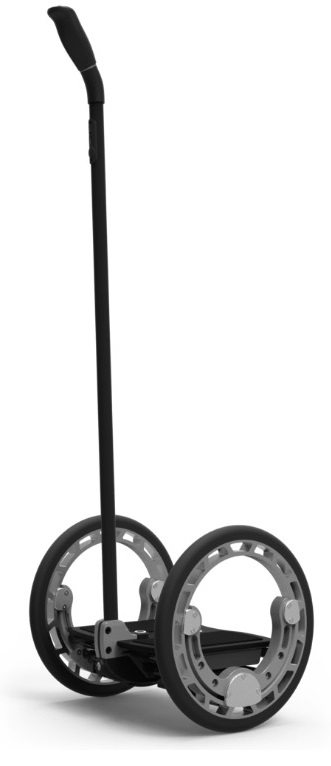
\includegraphics[width=.5\linewidth]{fig_01}
\end{marginfigure}


\section*{Mise en situation}
\ifprof
\else
L’exosquelette est un appareil qui apporte à un être humain des capacités qu’il ne possède pas ou qu’il a perdues à cause d’un accident. Ce type d’appareil peut permettre à une personne de soulever des charges lourdes et diminuer considérablement les efforts à fournir sans la moindre fatigue. Après avoir revêtu un exosquelette adapté à sa morphologie et à sa taille, l’utilisateur peut faire ses mouvements en bénéficiant
d’une grande fluidité.


On donne dans la figure ci-dessous, la modélisation cinématique retenue dans le but de simuler le comportement de l'exosquelette.


\begin{figure*}[h!]
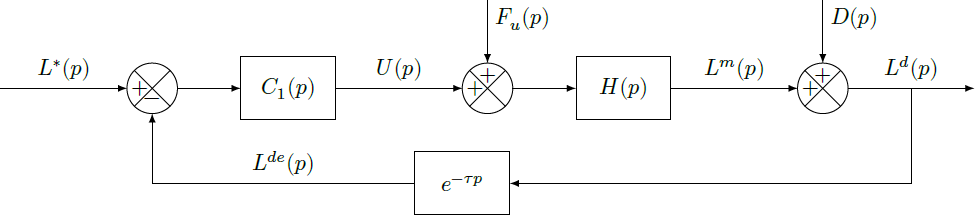
\includegraphics[height = 4cm]{fig_03}
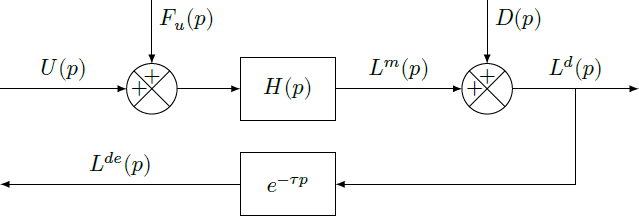
\includegraphics[height = 4cm]{fig_02}
\hfill%\textit{}
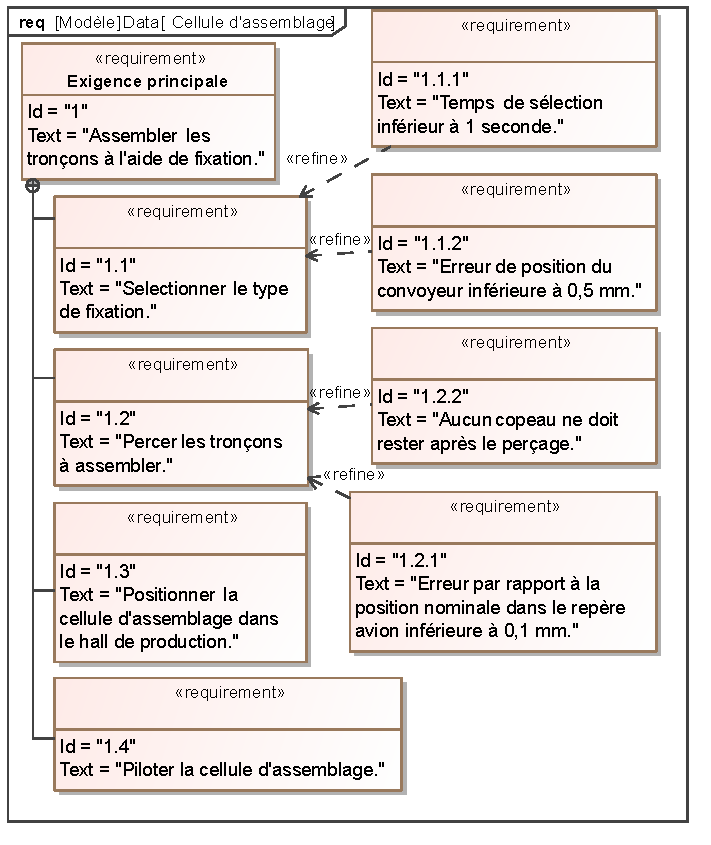
\includegraphics[height = 4cm]{Exigences}
\end{figure*}

\fi

\subsection*{Gestion du mouvement vertical}

\begin{obj}
Déterminer les réglages de la commande asservie des moteurs genou droit et gauche permettant d’assurer un mouvement vertical ne déséquilibrant pas le porteur de l’exosquelette puis valider les performances attendues listées par le cahier des charges.
\end{obj}


\ifprof
\else

\begin{marginfigure}
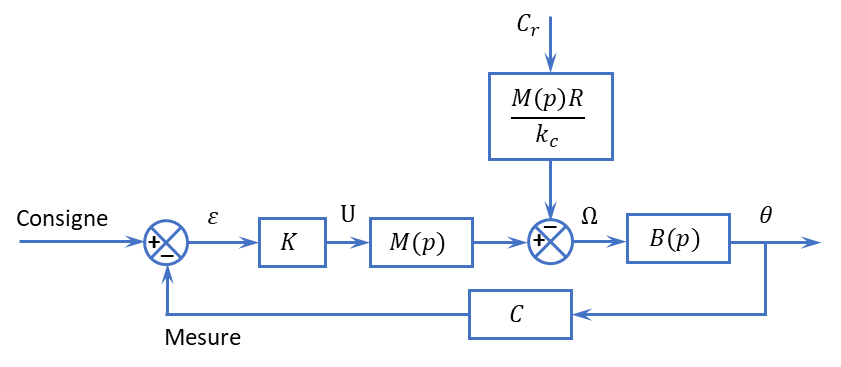
\includegraphics[width=\linewidth]{fig_06}
\end{marginfigure}

La demande de mouvement de l’utilisateur de l’exosquelette se traduit par une consigne de vitesse de type
trapézoïdal pour le mouvement vertical. À l’aide du modèle articulaire inverse cette
demande se traduit finalement en consigne de position des axes moteur genou gauche et droit. Cette consigne de position du moteur représentée à la figure suivante montre des parties qui peuvent être approchées par des constantes,
des rampes et des paraboles.


%Selon le cahier des charges, pour assurer une bonne synchronisation des axes, l’exigence de précision statique suite à une entrée de type échelon, de type rampe ou de type accélération doit être inférieure à 1\%.
Le premier modèle défini figure suivante est adopté pour chaque axe.


\begin{center}
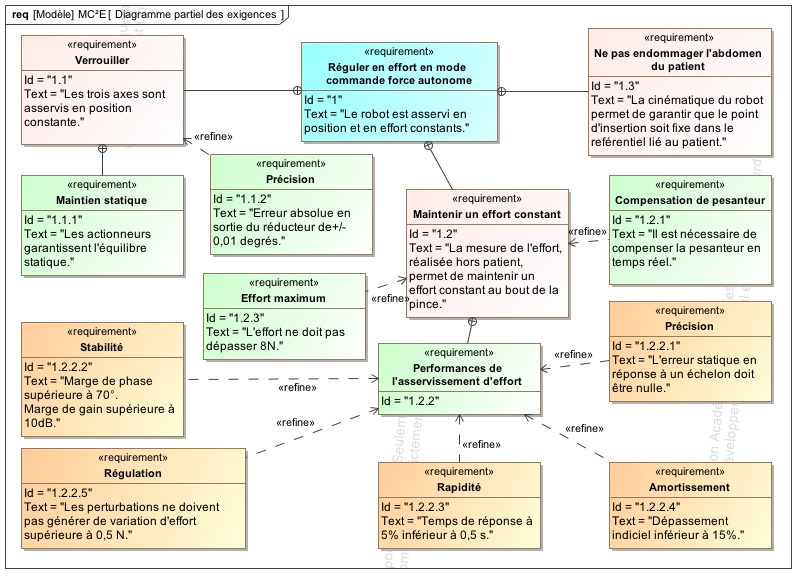
\includegraphics[width=\linewidth]{fig_05}
%\textit{}
\end{center}

\marginnote[-2cm]{
\textbf{Notations : }
\begin{itemize}
\item $\theta_{mC}(p)$ consigne de position de l’axe moteur (variable temporelle : $\theta_{mC}(t)$ en rad);
\item $\theta_{m}(p)$ position de l’axe moteur (variable temporelle : $\theta_{m}(t)$ en rad);
\item $C_{mC}(p)$ consigne de couple moteur (variable temporelle : $c_{mC}(t)$ en Nm);
\item $C_{m}(p)$ couple moteur (variable temporelle : $c_{m}(t)$ en Nm);
\item $C_{r}(p)$ couple résistant perturbateur (variable temporelle : $c_{r}(t)$ en Nm);
\item $K_1$ gain proportionnel du correcteur de l’asservissement de position (en $\text{s}^{-1}$);
\item $\Omega_{mC}(p)$ consigne de vitesse de l’axe moteur (variable temporelle : $\Omega_{mC}(t)$ en $\text{rad s}^{-1}$);
\item $\Omega_{m}(p)$ vitesse de l’axe moteur (variable temporelle : $\Omega_{m}(t)$ en  $\text{rad s}^{-1}$);
\item $C_{\Omega}(p)$ correcteur de l’asservissement de vitesse;
\item $M_C(p)$ modélise la boucle d’asservissement en couple de la machine électrique, considérée parfaite au vu de sa dynamique par rapport aux autres boucles : $M_C(p)=1$; 
\item $J$ moment d’inertie de l’ensemble en mouvement, rapporté au niveau de l’axe moteur;
\item $f$ coefficient de frottements visqueux équivalent pour l’ensemble en mouvement.
\end{itemize}}


Le correcteur est de la forme : $C_{\Omega}(p)=K_2 \left( \dfrac{Jp +f}{Jp}\right)$. 

En utilisant le schéma-blocs précédent, on peut constater que : 
\begin{itemize}
\item l'écart est défini par la variable $\varepsilon(t) = \theta_{mC}(t)-\theta_m(t)$;
\item l'erreur entre l’entrée et la sortie est définie par la variable $\mu(t)= \theta_{mC}(t)-\theta_m(t)$.
\end{itemize}

Étant donné que le modèle utilisé est à retour unitaire, l’écart $\varepsilon(t)$ est égal à l’erreur $\mu(t)$. 
%La précision statique du système est définie par les paramètres suivants :
%\begin{itemize}
%\item $\varepsilon_p = \lim\limits_{t\to \infty} \varepsilon(t)$ suite à une entrée de type échelon unitaire $\theta_{mC}(t)=u(t)$, $\theta_{mC}(p)=\dfrac{1}{p}$, appelée erreur de position;
%\item $\varepsilon_v = \lim\limits_{t\to \infty} \varepsilon(t)$ suite à une entrée de type rampe unitaire $\theta_{mC}(t)=tu(t)$, $\theta_{mC}(p)=\dfrac{1}{p^2}$, appelée erreur de traînage;
%\item $\varepsilon_a = \lim\limits_{t\to \infty} \varepsilon(t)$ suite à une entrée de type accélération $\theta_{mC}(t)=\dfrac{t^2}{2}u(t)$, $\theta_{mC}(p)=\dfrac{1}{p^3}$, appelée erreur en accélération.
%\end{itemize}

\begin{hypo}
Le couple résistant évolue lentement au regard de la dynamique de l’asservissement, ce qui permet de considérer
pour la suite de l’étude $C_r(p)=0$.
\end{hypo}

\fi

\question{Déterminer la grandeur physique de la consigne et la grandeur physique asservie à partir du modèle multiphysique présenté plus bas et préciser leurs unités de base dans le système international d’unités (SI).}
\ifprof
\begin{corrige}~\\
Il s'agit d'un asservissement en position. 

\begin{center}
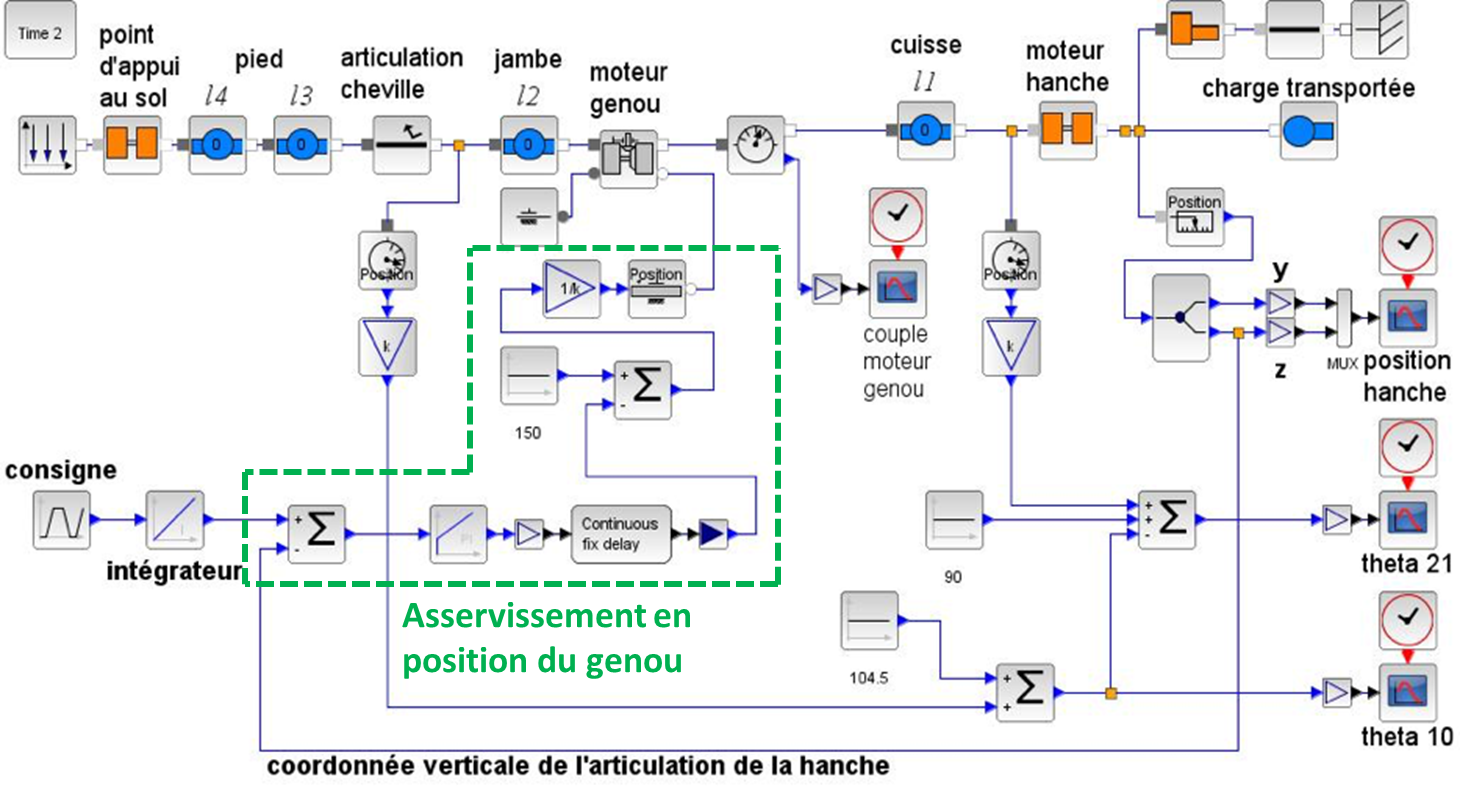
\includegraphics[width=\linewidth]{cor_01}
\end{center}
\end{corrige}

\else
\fi


\question{Exprimer $H_{\Omega}(p)=\dfrac{\Omega_m(p)}{\Omega_{mC}(p)}$
en fonction de $J$, $K_2$ et $p$.}
\ifprof
\begin{corrige}
En faisant l'hypothèse que le couple perturbateur est nul, on a :
$H_{\Omega}(p)=\dfrac{\Omega_m(p)}{\Omega_{mC}(p)}=\dfrac{C_{\Omega}(p)M_C(p)\dfrac{1}{Jp+f}}{1+C_{\Omega}(p)M_C(p)\dfrac{1}{Jp+f}}$. En conséquences : 
$H_{\Omega}(p)=\dfrac{K_2}{Jp+ K_2 } = \dfrac{1}{\dfrac{Jp}{C K_2}+1 } $.

\end{corrige}
\else
\fi

\question{Exprimer $\varepsilon(p)$ en fonction de $\theta_{mC}(p)$, $H_{\Omega}(p)$, $K_1$ et $p$.}
\ifprof

\begin{corrige}
D'une part, $\varepsilon(p)=\theta_{mC}(p)-\theta_{m}(p)$. D'autre part, 
$\theta_{m}(p) =H_{\Omega}(p) \dfrac{K_1}{p} \varepsilon(p)$. Par suite, 
$\varepsilon(p)=\theta_{mC}(p)-H_{\Omega}(p) \dfrac{K_1}{p}\varepsilon(p) $ 
$\Leftrightarrow \varepsilon(p)\left( 1+H_{\Omega}(p) \dfrac{K_1}{p}\right)= \theta_{mC}(p)$. 
En conséquences, $\varepsilon(p)=\dfrac{ \theta_{mC}(p)}{ 1+H_{\Omega}(p) \dfrac{K_1}{p}}$.
\end{corrige}
\else
\fi

\ifprof
\else
\begin{methode} On peut définir l'erreur de position $\varepsilon_p$ par $\varepsilon_p=\lim\limits_{t \to +\infty} \varepsilon(t)=\lim\limits_{p \to 0} p\varepsilon(p)$ avec  $\theta_{mC}(p)=\dfrac{1}{p}$ (entrée échelon).
\end{methode}
\fi

\question{Déterminer l’erreur de position $\varepsilon_p$ puis l’erreur de traînage $\varepsilon_v$. Conclure sur la valeur de $K_1$ pour satisfaire
à l’exigence d’erreur en traînage.}

\ifprof
\begin{corrige}
On a :
\begin{itemize}
\item $\varepsilon_p = \lim\limits_{t\to \infty} \varepsilon(t)= \lim\limits_{p\to 0} p\varepsilon(p) $ $= \lim\limits_{p\to 0} p \dfrac{ 1}{ 1+H_{\Omega}(p) \dfrac{K_1}{p}} \dfrac {1}{p}$
$= \lim\limits_{p\to 0} \dfrac{ 1}{ 1+\dfrac{1}{\dfrac{Jp}{C_{\Omega} K_2}+1 } \dfrac{K_1}{p}} = 0$ (ce qui était prévisible pour un système de classe 1);
\item $\varepsilon_v = \lim\limits_{t\to \infty} \varepsilon(t)= \lim\limits_{p\to 0} p\varepsilon(p) $ $= \lim\limits_{p\to 0} p \dfrac{ 1}{ 1+H_{\Omega}(p) \dfrac{K_1}{p}} \dfrac {1}{p^2}$
$= \lim\limits_{p\to 0} \dfrac{ 1}{ 1+\dfrac{1}{\dfrac{Jp}{C_{\Omega} K_2}+1 } \dfrac{K_1}{p}}\dfrac {1}{p} $
$= \lim\limits_{p\to 0} \dfrac{ 1}{ p+\dfrac{1}{\dfrac{Jp}{C_{\Omega} K_2}+1 } K_1}= \dfrac{1}{K_1}$ (ce qui était prévisible pour un système de classe 1 et de gain $K_1$ en BO).
\end{itemize}

Ainsi, pour avoir une erreur de traînage inférieure à 1\%, il faut $\dfrac{1}{K_1}<0,01$ et $K_1 >100$.
\end{corrige}
\else
\fi







\question{Déterminer l’erreur en accélération et conclure quant au respect du cahier des charges.}


\ifprof

\begin{corrige}
En raisonnant de même, on a :
 $\varepsilon_a = \lim\limits_{t\to \infty} \varepsilon(t)= \lim\limits_{p\to 0} p\varepsilon(p) $ $= \lim\limits_{p\to 0} p \dfrac{ 1}{ 1+H_{\Omega}(p) \dfrac{K_1}{p}} \dfrac {1}{p^3}$
$= \lim\limits_{p\to 0} \dfrac{ 1}{ 1+\dfrac{1}{\dfrac{Jp}{C_{\Omega} K_2}+1 } \dfrac{K_1}{p}}\dfrac {1}{p^2} = 0$
$= \lim\limits_{p\to 0} \dfrac{ 1}{ p^2+\dfrac{p}{\dfrac{Jp}{C_{\Omega} K_2}+1 } K_1}= \infty$ (ce qui était prévisible pour un système de classe 1).


Ainsi, le correcteur choisi ne permet pas de vérifier le cahier des charges. 
\end{corrige}
\else
\fi

\ifprof
\else
Pour satisfaire l’exigence d’une erreur en accélération inférieure à 1\%, le second modèle avec anticipation de la
vitesse est adopté avec $H_{\Omega}(p)=\dfrac{1}{1+Tp}$ et $T=\SI{33}{ms}$.

\begin{center}
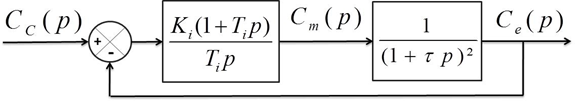
\includegraphics[width=\linewidth]{fig_08}
%\textit{}
\end{center}
\fi

\question{Exprimer $\varepsilon(p)$ en fonction de $\theta_{mC}(p)$, $T$, $K_1$, $K_3$ et $p$.}
\ifprof

\begin{corrige}
En utilisant le schéma-blocs, on a : 
\begin{itemize}
\item 
$ \varepsilon(p)=\theta_{mC}(p)-\theta_{m}(p)$;
\item  $\Omega_{mC}(p)=K_3 p \theta_{mC}(p) + K_1 \varepsilon(p)$;
\item $\theta_m(p)=\Omega_{mC}(p) \dfrac{1}{p}\dfrac{1}{1+Tp}$. 
\end{itemize}
On a donc : 
$ \varepsilon(p)=\theta_{mC}(p)-\Omega_{mC}(p) \dfrac{1}{p}\dfrac{1}{1+Tp}$ 
$= \theta_{mC}(p)- 
\left(K_3 p \theta_{mC}(p) + K_1 \varepsilon(p)  \right)
\dfrac{1}{p \left( 1+Tp\right)}$
$= \theta_{mC}(p)- 
 \dfrac{K_3 p }{p \left( 1+Tp\right)} \theta_{mC}(p)
-  \dfrac{K_1 }{p \left( 1+Tp\right)} \varepsilon(p)
$. 

On a alors 
$
\varepsilon(p)  \left(1+ \dfrac{K_1 }{p \left( 1+Tp\right)} \right)
=  \theta_{mC}(p)\left(1-  \dfrac{K_3}{ 1+Tp}\right)$

$\Leftrightarrow
\varepsilon(p)  \dfrac{p \left( 1+Tp\right)+K_1 }{p \left( 1+Tp\right)} 
=  \theta_{mC}(p)  \dfrac{ 1+Tp-K_3  }{ 1+Tp}
$.

Enfin,  
$\varepsilon(p) = \theta_{mC}(p)\dfrac{p\left( 1+Tp-K_3\right) }{p \left( 1+Tp\right)+K_1}
$.
\end{corrige}

\else

Le second modèle avec anticipation de la figure précédente n’a pas d’incidence sur la valeur de l’erreur de position.
\fi


\question{Exprimer l’erreur de traînage et déterminer la valeur de $K_3$ permettant l’annuler cette erreur.}

\ifprof

\begin{corrige}
$\varepsilon_v = \lim\limits_{t\to \infty} \varepsilon(t)= \lim\limits_{p\to 0} p\varepsilon(p) $ 
$= \lim\limits_{p\to 0} p \dfrac{p\left( 1+Tp-K_3\right) }{p \left( 1+Tp\right)+K_1} \dfrac {1}{p^2}$
$= \lim\limits_{p\to 0}  \dfrac{\left( 1+Tp-K_3\right) }{p \left( 1+Tp\right)+K_1}$
$=\dfrac{1-K_3}{K_1}$.


Au final, pour annuler l'erreur de traînage, on doit avoir $K_3=1$.
\end{corrige}
\else
\fi
\question{Exprimer et déterminer l’erreur d’accélération en prenant les valeurs de $K_3$ et de $K_1$ déterminées
précédemment. Conclure quant au respect du cahier des charges.}\\

\ifprof
\begin{corrige}
On a : 
$\varepsilon_a = \lim\limits_{t\to \infty} \varepsilon(t)= \lim\limits_{p\to 0} p\varepsilon(p) $ 
$= \lim\limits_{p\to 0} p \dfrac{p\left( 1+Tp-K_3\right) }{p \left( 1+Tp\right)+K_1} \dfrac {1}{p^3}$
$= \lim\limits_{p\to 0} \dfrac{\left( 1+Tp-K_3\right) }{p \left( 1+Tp\right)+K_1} \dfrac {1}{p}$. En prenant $K_3=1$ et $K_1=100$, on obtient :
$\varepsilon_a = \dfrac{ T}{p \left( 1+Tp\right)+100}=\dfrac{33\times 10^{-3}}{100} $.
L'erreur est donc de $33\times 10^{-5}$. Le cahier des charges est donc validé. 

\end{corrige}
\else
\fi

\subsection*{Synthèse}
\question{En utilisant la figure ci-dessous, conclure sur les actions qui ont mené à une validation du cahier des charges.}\\

\ifcolle
\else
\ifprof
\else
\marginnote{
\begin{solution}
\begin{enumerate}[wide, labelwidth=!, labelindent=0pt]
\item Asservissement en position.
\item $H_{\Omega}(p)= \dfrac{K_2}{Jp+K_2}$.%{1}/\left(\dfrac{Jp}{C_{\Omega} K_2}+1 \right) $.
\item $\varepsilon(p)=\dfrac{ \theta_{mC}(p)}{1+H_{\Omega}(p) \dfrac{K_1}{p}}$
\item $\varepsilon(p)= 0, \varepsilon_v = \dfrac{1}{K_1}$   et $K_1 >100$.
\item $\varepsilon_a = \infty$.
\item $\varepsilon(p) = \theta_{mC}(p)\dfrac{p\left( 1+Tp-K_3\right) }{p \left( 1+Tp\right)+K_1} $.
\item $\varepsilon_v =\dfrac{1-K_3}{K_1}$, $K_3=1$.
\item $\varepsilon_a = \dfrac{33\times 10^{-3}}{100} $. Le cahier des charges est donc validé. 
\end{enumerate}
\end{solution}}
\fi
\fi


\ifprof
\begin{center}
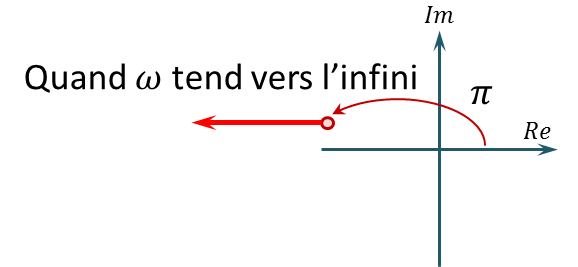
\includegraphics[width=\linewidth]{cor_02}
%\textit{}
\end{center}

\else
\begin{center}
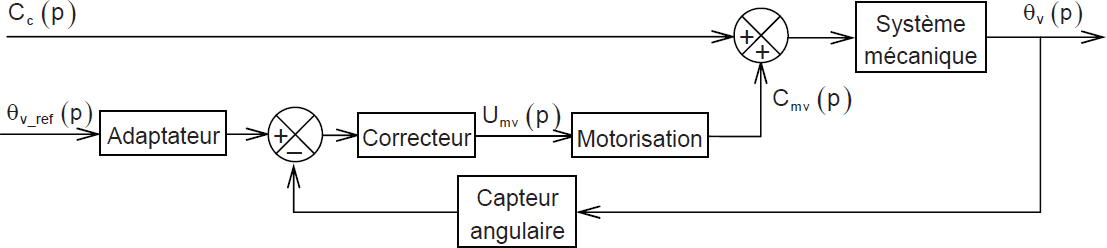
\includegraphics[width=\linewidth]{fig_10}
%\textit{}
\end{center}
\fi
